\documentclass[conference]{IEEEtran}
% CAMERA-READY step 1 of 3: required, or IEEEtran silently ignores
% \IEEEpubid in conference mode ("locked out" warning in the .log).
%\IEEEoverridecommandlockouts

% ── Encoding & Fonts ─────────────────────────────────────────────
\usepackage[T1]{fontenc}
\usepackage[utf8]{inputenc}

% ── Mathematics ──────────────────────────────────────────────────
\usepackage{amsmath,amssymb,amsthm}

% ── Graphics & Figures ───────────────────────────────────────────
\usepackage{graphicx}
\usepackage{tikz}
\usetikzlibrary{shapes.geometric,arrows.meta,positioning,calc}
\usepackage{pgfplots}
\pgfplotsset{compat=1.18}

% ── Tables ───────────────────────────────────────────────────────
\usepackage{booktabs}
\usepackage{array}

% ── Hyperlinks & References ───────────────────────────────────────
\usepackage[hidelinks]{hyperref}
\usepackage{cite}
\usepackage{url}
\hypersetup{
  pdftitle={ARES: A Formal Reliability Framework for Detecting Anomalous Behaviour in Agentic AI Systems},
  pdfauthor={Mohammad Makchudul Alam; Md. Redowan Z. Anik; Sabrein S. E. el Bodour; Anca Delia Jurcut},
  pdfsubject={Agentic AI reliability, hallucination, SOC, IEEE ISAIA 2026},
  pdfkeywords={ARES; agentic AI reliability; SKC mismatch; Agent Reliability Score; Epistemic Gap; anomaly detection; LLM hallucination}
}

% ── Misc ─────────────────────────────────────────────────────────
\usepackage{xcolor}
\usepackage{balance}
\usepackage{microtype}
\usepackage{enumitem}

% ── Theorem environments ─────────────────────────────────────────
\newtheorem{definition}{Definition}
\newtheorem{theorem}{Theorem}
\newtheorem{proposition}{Proposition}
\newtheorem{hypothesis}{Hypothesis}

% ── Custom notation ───────────────────────────────────────────────
\newcommand{\A}{\mathcal{A}}
\newcommand{\T}{\mathcal{T}}
\newcommand{\Sk}{\mathcal{S}}
\newcommand{\K}{\mathcal{K}}
\newcommand{\CC}{\mathcal{C}}
\newcommand{\R}{\mathcal{R}}
\newcommand{\E}{\mathcal{E}}
\newcommand{\ARS}{\mathrm{ARS}}
\newcommand{\bw}{\mathbf{w}}
\newcommand{\bdelta}{\boldsymbol{\delta}}
\newcommand{\norm}[1]{\left\lVert#1\right\rVert}
\newcommand{\Tage}{\mathcal{T}_{\mathrm{age}}}

% ── Framework name macros ─────────────────────────────────────────
\newcommand{\ARES}{\textsc{ARES}}
\newcommand{\ARESBench}{\textsc{ARES-Bench}}
\newcommand{\SAFK}{\textsc{SOCAgentFailure-1K}}

% ─────────────────────────────────────────────────────────────────
\begin{document}

\title{ARES: A Formal Reliability Framework for Detecting Anomalous Behaviour in Agentic AI Systems}

\author{%
\IEEEauthorblockN{1\textsuperscript{st} Mohammad Makchudul Alam}
\IEEEauthorblockA{\textit{CTI, BGD e-GOV CIRT}\\
\textit{DNS Research Lab}\\
(www.dnsresearchlabs.ucd.ie) \\
Dhaka, Bangladesh \\
engrarifcce@gmail.com \\
\small }
\and
\IEEEauthorblockN{2\textsuperscript{nd} Md.~Redowan Z.\ Anik}
\IEEEauthorblockA{\textit{Cyber Threat Intelligence} \\
\textit{BGD e-GOV CIRT}\\
Dhaka, Bangladesh \\
redowanzanik@gmail.com}
\and
\IEEEauthorblockN{3\textsuperscript{rd} Sabrein S.~E.~el Bodour}
\IEEEauthorblockA{\textit{Cyber Threat Intelligence} \\
\textit{BGD e-GOV CIRT}\\
Dhaka, Bangladesh \\
sabreinserag@gmail.com}
\and
\IEEEauthorblockN{4\textsuperscript{th} Anca Delia Jurcut}
\IEEEauthorblockA{\textit{Sch.\ of Computer Science} \\
\textit{Univ.\ College Dublin}\\
Dublin, Ireland \\
anca.jurcut@ucd.ie}
}

\maketitle

% ── CAMERA-READY step 2 of 3: IEEE copyright notice ──────────────
% ISAIA 2026 will supply the conference ISBN and confirm which of the
% four IEEE copyright lines applies. Uncomment ONE line below, insert
% the ISBN, and also uncomment step 1 (above) and step 3 (the
% \IEEEpubidadjcol in sections/01_introduction.tex). Verified recipe:
% the notice then sets at the foot of column 1 on page 1 and the text
% reflows to make room, with the paper still at 6 pages.
%
% 1. Standard (most authors):
%\IEEEpubid{\makebox[\columnwidth]{979-8-XXXX-XXXX-X/26/\$31.00~\copyright2026 IEEE \hfill}\hspace{\columnsep}\makebox[\columnwidth]{}}
%
% 2. All authors are US government employees:
%\IEEEpubid{\makebox[\columnwidth]{U.S. Government work not protected by U.S. copyright \hfill}\hspace{\columnsep}\makebox[\columnwidth]{}}
%
% 3. Crown copyright (UK/Canada/Australia government):
%\IEEEpubid{\makebox[\columnwidth]{979-8-XXXX-XXXX-X/26/\$31.00~\copyright2026 Crown \hfill}\hspace{\columnsep}\makebox[\columnwidth]{}}
%
% 4. European Union:
%\IEEEpubid{\makebox[\columnwidth]{979-8-XXXX-XXXX-X/26/\$31.00~\copyright2026 European Union \hfill}\hspace{\columnsep}\makebox[\columnwidth]{}}
% ─────────────────────────────────────────────────────────────────

\begin{abstract}
Autonomous AI agents deployed in Security Operations Centres (SOCs) are
susceptible to failures arising from mismatches between task demands and
agent capabilities across skill, knowledge, and capability dimensions.
Despite growing deployment, no formal reliability model that quantifies
this mismatch and predicts failure risk before execution has, to the best
of our knowledge, been proposed. We present ARES (Agentic Reliability
Evaluation for Security systems), a formal reliability framework that
introduces three components: a five-dimensional
Skill--Knowledge--Capability (SKC) mismatch vector; a learnable Agent
Reliability Score (ARS) with task-class-specific weights; and an
Epistemic Gap metric that formalises the hallucination precondition as
confident ignorance. Experimental validation on 1,000 agent execution
traces demonstrates that knowledge mismatch is the dominant predictor of
hallucination (bucket-aggregated correlation 0.92 at $p < 0.0001$,
point-biserial correlation 0.34 at the record level), the ARS threshold
generalises across five threat classes (held-out test F1 of 0.96), and
the Epistemic Gap provides an interpretable decomposition of
false-negative risk into knowledge and calibration components.
The framework provides an initial formal foundation for pre-deployment
reliability screening and runtime anomaly detection in agentic AI systems.

\end{abstract}

\begin{IEEEkeywords}
ARES framework, agentic AI reliability, SKC mismatch, Agent Reliability Score,
epistemic gap, anomaly detection, LLM hallucination
\end{IEEEkeywords}

\section{Introduction}

The deployment of autonomous AI agents in Security Operations Centres
(SOCs) is accelerating rapidly. Frameworks such as LangGraph~\cite{langgraph2024},
AutoGen~\cite{wu2023autogen}, and CrewAI~\cite{crewai2024} enable LLM-based
agents to perform threat detection, incident triage, and response
recommendation with minimal human supervision. Yet a fundamental gap persists
in our understanding of these systems: \textit{when do they fail, why do they
fail, and how severely?}

The security community has invested heavily in measuring agent
capabilities (detection accuracy, response speed, ATT\&CK coverage) but
much less in the conditions under which agents produce incorrect,
incomplete, or misleading outputs. This asymmetry carries
serious consequences: a false negative allows an intrusion to persist, a
hallucinated threat attribution poisons shared intelligence feeds, and an
agent paralysed by missing tool access delays incident response beyond
regulatory thresholds.

We identify the core reliability challenge as the
\textit{Skill--Knowledge--Capability (SKC) Mismatch}: the gap between what
a security task demands and what an agent can deliver across several
dimensions. To the best of our knowledge, no existing formal framework ties this
capability mismatch to failure risk in a quantifiable, pre-execution way.

\textbf{Gap in existing work.}
Classical dependability theory~\cite{avizienis2004} provides rigorous fault
taxonomies for conventional software but predates LLM agents and has no
concept of epistemic uncertainty or knowledge currency. Hallucination
research~\cite{huang2023hallucination} analyses LLM reasoning failures but
ignores operational context. AgentBench~\cite{liu2023agentbench} benchmarks
agent task performance without modelling capability constraints or failure
conditions.

\textbf{Contribution.}
We present \ARES{} (Agentic Reliability Evaluation for Security systems),
a compact formal framework for estimating reliability risk in agentic AI
before and during cybersecurity task execution. The conference contribution
is narrow:
\begin{enumerate}[noitemsep, leftmargin=*]
  \item A \textbf{five-dimensional SKC mismatch model} that quantifies the
    gap between agent capability and task demand, producing a learnable
    Agent Reliability Score (ARS) usable as a pre-execution screening
    signal.
  \item An \textbf{Epistemic Gap metric} that formalises the hallucination
    precondition as confident ignorance: the interaction between knowledge
    deficit and miscalibrated confidence.
  \item An \textbf{analytical validation} showing that knowledge
    mismatch dominantly predicts hallucination, the ARS threshold
    generalises across threat classes, and the Epistemic Gap provides an
    interpretable decomposition of false-negative risk into knowledge
    and calibration components.
\end{enumerate}
\ARES{} contributes to intelligent systems research by providing a
reliability-oriented representation and decision framework for autonomous
agents operating under incomplete knowledge and capability constraints.
A cascade reliability bound for tightly-coupled multi-agent pipelines and
a temporal-drift model for knowledge ageing are reported as supporting
results.

The remainder of this paper is organised as follows. Section~\ref{sec:related}
surveys related work. Section~\ref{sec:framework} presents the formal SKC
reliability framework. Section~\ref{sec:epistemic} introduces the Epistemic
Gap. Section~\ref{sec:experimental} provides experimental validation.
Section~\ref{sec:discussion} discusses implications, and
Section~\ref{sec:conclusion} concludes.

\section{Related Work}
\label{sec:related}

\textbf{AI dependability and fault taxonomies.}
Avizienis et al.~\cite{avizienis2004} define the foundational taxonomy of
faults, errors, and failures, but it targets conventional deterministic
software: it has no concept of epistemic uncertainty, knowledge coverage,
or reasoning-chain validity, and assumes a complete specification against
which correctness can be verified---an assumption that does not hold for
LLM agents operating with incomplete, potentially stale knowledge.

Humbatova et al.~\cite{humbatova2020} taxonomise real-world bugs in deep
learning systems across model, data, and training faults, but neither the
security domain nor the agentic tool-use paradigm is addressed. Their
taxonomy captures \textit{implementation} faults; \ARES{} captures
\textit{operational} mismatches where the agent is correctly implemented
but insufficiently equipped for the task.

\textbf{LLM hallucination and confidence calibration.}
Huang et al.~\cite{huang2023hallucination} survey hallucination in LLMs but
treat it as a property of the model in isolation, not of the
\textit{operational context} (tool availability, task complexity, knowledge
freshness) that characterises SOC deployments; nor does this literature
examine the multi-agent setting where one agent's hallucination propagates
to downstream reasoning stages.

Guo et al.~\cite{guo2017calibration} show modern neural networks are
systematically overconfident on out-of-distribution inputs. Existing
calibration work measures miscalibration globally; our Epistemic Gap
(Section~\ref{sec:epistemic}) instead targets the specific case where
miscalibration coincides with the point of greatest knowledge weakness.

\textbf{Agent benchmarking and security AI.}
AgentBench~\cite{liu2023agentbench} is the closest existing work to our
evaluation approach, providing a multi-environment benchmark for LLM agents
across web navigation, code execution, and game playing tasks. However,
AgentBench includes no security environment, does not model capability
constraints, and does not support systematic mismatch injection.
PentestGPT~\cite{deng2023pentest} evaluates LLM penetration testing
capabilities, but does not model the conditions under which agents
produce misleading outputs.

The broader AI in cybersecurity literature~\cite{apruzzese2023} catalogues
AI applications across the security lifecycle but explicitly identifies
agent reliability as an open problem. All such work characterises
\textit{what agents can do}, not \textit{how and why they fail}.

\textbf{Contemporary agent-failure taxonomies and benchmarks.}
Two 2024--2025 efforts overlap with \ARES{}'s scope and require
explicit positioning. MAST~\cite{cemri2025mast} derives 14
failure modes from $1{,}600{+}$ annotated traces across seven
multi-agent frameworks and clusters them into system-design,
inter-agent-misalignment, and task-verification categories.
MAST is domain-agnostic and descriptive; \ARES{} is security-specific
and predictive, providing a \textit{pre-execution} reliability
score (ARS) and a formal cascade bound that MAST documents
empirically as ``cascade amplification'' without formalisation.
AgentDojo~\cite{debenedetti2024agentdojo} provides a dynamic
environment with 629 prompt-injection test cases for adversarial
evaluation. \ARES{} covers the orthogonal \textit{non-adversarial}
failure surface: agents failing because capability does not match
task demand, independent of any active attacker. The 2025
hallucination benchmark suite HalluLens~\cite{bang2025hallulens}
measures LLM factual fabrication on generic QA with retrieval
probes, and a concurrent broad survey of LLM-agent
hallucination~\cite{llmagent_halluc_survey2025} catalogues
taxonomy and mitigation approaches across $70{+}$ studies. Both
establish that hallucination is a cross-domain agent failure
mode; \ARES{} contributes the piece that is missing from
this literature: connecting hallucination rate to the specific
capability dimensions of a security task, and modelling cascade
amplification analytically rather than descriptively. At the
application-governance layer, the OWASP Top~10 for Agentic
Applications~\cite{owasp2026agentic} names capability
over-provisioning, tool misuse, and confident hallucination as
top-tier risks; these correspond precisely to $\delta_C$
over-provision, $\delta_C$ and $\delta_R$ interaction, and
Epistemic-Gap failures in our framework.

\textbf{Gap summary.}
Table~\ref{tab:related_isaia} summarises the coverage landscape. To the
best of our knowledge, three gaps are simultaneously unaddressed:
(i)~no formal model covers the full SKC failure surface including
temporal drift and epistemic gap; (ii)~no framework connects capability
mismatch to failure probability quantitatively; and (iii)~no model
predicts hallucination from the interaction of knowledge deficit and
confidence miscalibration. \ARES{} addresses all three.

\begin{table}[t]
\caption{Related Work Coverage Comparison}
\label{tab:related_isaia}
\centering
\footnotesize
\setlength{\tabcolsep}{3pt}
\begin{tabular}{lccccc}
\toprule
\textbf{Work} & \textbf{Formal} & \textbf{Security} & \textbf{Failure} & \textbf{Epistemic} & \textbf{Cascade} \\
& \textbf{Model} & \textbf{Domain} & \textbf{Taxonomy} & \textbf{Gap} & \textbf{Model} \\
\midrule
Avizienis~\cite{avizienis2004}   & \checkmark & -- & \checkmark & -- & -- \\
Huang~\cite{huang2023hallucination} & -- & -- & Partial & -- & -- \\
Humbatova~\cite{humbatova2020}   & -- & -- & \checkmark & -- & -- \\
AgentBench~\cite{liu2023agentbench} & -- & -- & -- & -- & -- \\
PentestGPT~\cite{deng2023pentest} & -- & \checkmark & -- & -- & -- \\
MAST~\cite{cemri2025mast}            & -- & -- & \checkmark & -- & Partial \\
AgentDojo~\cite{debenedetti2024agentdojo} & -- & -- & -- & -- & -- \\
\textbf{\ARES{}} & \checkmark & \checkmark & \checkmark & \checkmark & \checkmark \\
\bottomrule
\end{tabular}
\end{table}

\section{ARES Reliability Framework}
\label{sec:framework}

We use \textit{agentic AI system} for the deployment-level entity (an
LLM-driven agent or pipeline operating in a SOC) and \textit{AI security
agent} for its formal model: the five-tuple object of
Definition~\ref{def:agent} that the framework reasons about.

\subsection{Agent and Task Profiles}

\begin{definition}[AI Security Agent]
\label{def:agent}
  An AI security agent $\A$ is a five-tuple:
  $\A = \langle \Sk, \K, \CC, \R, \Tage \rangle$
  where $\Sk$ is a finite set of skills (executable procedures),
  $\K$ is a knowledge base of threat-relevant facts,
  $\CC$ is a set of capabilities (tool and API access),
  $\R$ denotes the reasoning engine, and
  $\Tage \in \mathbb{R}_{\geq 0}$ is the agent's knowledge age in days.
\end{definition}

\begin{definition}[Task Requirement Profile]
  A security task $\T$ is a four-tuple:
  $\T = \langle \Sk^*, \K^*, \CC^*, y^* \rangle$
  where $\Sk^*$, $\K^*$, $\CC^*$ are the minimum required subsets and
  $y^* \in \mathcal{Y}$ is the ground-truth correct output.
\end{definition}

\subsection{Mismatch Indicators}

For each capability dimension, we define a normalised mismatch indicator
$\delta \in [0,1]$ where 0 denotes full coverage and 1 denotes total
mismatch:

\begin{definition}[Skill Mismatch]
  $\delta_S(\A, \T) = |\Sk^* \setminus \Sk| \;/\; |\Sk^*|$
\end{definition}

\begin{definition}[Knowledge Mismatch]
  $\delta_K(\A, \T) = |\K^* \setminus \K| \;/\; |\K^*|$,
  measured as subgraph cardinality over the MITRE ATT\&CK TTP nodes
  required by the task's kill-chain.
\end{definition}

\begin{definition}[Capability Mismatch]
  $\delta_C(\A, \T) = |\CC^* \setminus \CC| \;/\; |\CC^*|$
\end{definition}

\begin{definition}[Reasoning Mismatch]
  $\delta_R(\A, \T) = 1 - \mathrm{Sim}(\hat{y}, y^*)$,
  where $\hat{y}$ is the agent's output and $\mathrm{Sim}(\cdot,\cdot)$ is
  a domain-appropriate similarity function (exact match for classification;
  semantic similarity for open-ended reports).
\end{definition}

\begin{definition}[Temporal Drift]
  $\delta_T(\A, \tau) = 1 - e^{-\lambda_\tau \cdot \Tage(\A)}$,
  where $\lambda_\tau > 0$ is the threat landscape volatility parameter for
  task class $\tau$, capturing the rate at which knowledge becomes outdated.
\end{definition}

The first three dimensions ($\delta_S$, $\delta_K$, $\delta_C$) and temporal
drift ($\delta_T$) are computable \textit{prior to task execution}. Only
$\delta_R$ requires post-hoc measurement. We therefore use ARS in two
modes: a pre-execution screening score $\ARS^{\mathrm{pre}}$ that drops
$\delta_R$ and re-normalises the remaining four weights to sum to one,
and a post-execution diagnostic score $\ARS$ that includes $\delta_R$
once the agent's output has been observed. Section~\ref{sec:experimental}
reports both.

\subsection{SKC Mismatch Vector and Agent Reliability Score}

\begin{definition}[SKC Mismatch Vector]
  $\bdelta(\A, \T) = [\delta_S,\ \delta_K,\ \delta_C,\ \delta_R,\ \delta_T]^\top \in [0,1]^5$
\end{definition}

\begin{definition}[Agent Reliability Score]
\label{def:ars}
  The Agent Reliability Score for agent $\A$ on task $\T$ of class $\tau$ is:
  \begin{equation}
    \ARS(\A, \T) = 1 - \bw_\tau^\top \bdelta(\A, \T)
    \label{eq:ars}
  \end{equation}
  where $\bw_\tau = [w_S, w_K, w_C, w_R, w_T]^\top$ is a task-class-specific
  weight vector with $\norm{\bw_\tau}_1 = 1$ and $w_i \geq 0$. A separate
  ridge regression is fit per task class on the training split, regressing
  the labelled per-record reliability outcome (binary anomaly flag) on the
  observed five-dimensional mismatch vector; the estimated coefficients are
  projected onto the simplex (clip negatives, $\ell_1$-normalise) to obtain
  $\bw_\tau$. ARS is clamped to $[0,1]$.
\end{definition}

Intuitively, ARS decreases when a task requires skills, knowledge, tools,
reasoning quality, or freshness that the agent lacks.

The task-class dependency of $\bw_\tau$ is a critical design choice.
Empirical results (Section~\ref{sec:experimental}) show that for APT
investigation, $w_K$ and $w_R$ dominate; for DDoS detection, $w_S$ and
$w_C$ lead. A universal weight vector would systematically misestimate
reliability across threat classes.

Table~\ref{tab:weights_isaia} reports the learned weight vectors, confirming
that $w_K$ is the highest mean-weight dimension ($\bar{w}_K = 0.30$),
reflecting the knowledge-intensive nature of threat analysis. The
task-class variability justifies the class-specific design.

\begin{table}[t]
\caption{Learned Weight Vectors $\bw_\tau$ per Task Class}
\label{tab:weights_isaia}
\centering
\footnotesize
\begin{tabular}{lrrrrr}
\toprule
\textbf{Task Class} & $w_S$ & $w_K$ & $w_C$ & $w_R$ & $w_T$ \\
\midrule
T1 Ransomware       & 0.18 & 0.35 & 0.22 & 0.17 & 0.08 \\
T2 Phishing         & 0.21 & 0.31 & 0.19 & 0.21 & 0.08 \\
T3 Insider Threat   & 0.15 & 0.27 & 0.36 & 0.15 & 0.07 \\
T4 DDoS             & 0.32 & 0.21 & 0.28 & 0.12 & 0.07 \\
T5 APT Intrusion    & 0.14 & 0.38 & 0.18 & 0.24 & 0.06 \\
\bottomrule
\end{tabular}
\end{table}

\subsection{Cascade Reliability for Multi-Agent Systems}

When agents are composed into a pipeline, failures propagate. We model
agent dependencies as a directed acyclic graph $G = (V, E, \mu)$ and
define cascade reliability as:
\begin{equation}
  \ARS_{\mathrm{cas}}(G, \T) = \prod_{(i,j) \in E}
    \!\left(1 - \mu_{ij} \cdot (1 - \ARS(\A_i, \T_i))\right)
  \label{eq:cascade}
\end{equation}
where $\mu_{ij} \in [0,1]$ is the coupling strength between agents.

\begin{theorem}[Cascade Reliability Bound]
\label{thm:cascade}
  Let $i^* \in V$ minimise $\ARS(\A_i, \T_i)$, write
  $r^* = \ARS(\A_{i^*}, \T_{i^*})$, and let
  $\mu^*_{\max} = \max\{\mu_{i^*j} : (i^*, j) \in E\}$ be the largest
  coupling on any outgoing edge of the weakest agent. If $i^*$ has at
  least one outgoing edge, then
  \begin{equation}
    \ARS_{\mathrm{cas}}(G, \T) \;\leq\; 1 - \mu^*_{\max}\,(1 - r^*).
    \label{eq:cascade_bound}
  \end{equation}
  In the fully-coupled case ($\mu^*_{\max} = 1$), this reduces to
  $\ARS_{\mathrm{cas}} \leq r^*$, so cascade reliability is bounded above
  by the weakest agent whenever that agent's output fully determines its
  successor's input.
\end{theorem}

\begin{proof}[Sketch]
The factor in \eqref{eq:cascade} associated with the outgoing edge of
$i^*$ achieving $\mu^*_{\max}$ equals $1 - \mu^*_{\max}(1 - r^*)$ and
lies in $[0,1]$, as do all other factors. The product of nonnegative
quantities each at most one is bounded above by any single factor,
yielding \eqref{eq:cascade_bound}. The case $\mu^*_{\max} = 1$ recovers
the weakest-link inequality. \qed
\end{proof}

Equation~\eqref{eq:cascade_bound} makes the role of coupling explicit:
partial coupling ($\mu < 1$) dilutes the upstream error and can keep
cascade reliability above $r^*$; full coupling collapses the bound onto
the weakest agent. The operational implication survives in either case:
multi-agent pipeline decomposition cannot improve reliability beyond the
weakest component when stages are tightly coupled.

\subsection{Anomaly Detection}

An agent execution is flagged as anomalous if:
\begin{equation}
  \Phi(\A, \T) = \mathbf{1}\!\left[\ARS(\A, \T) < \theta \;\lor\;
    \E(\A, \T) > \epsilon\right]
  \label{eq:anomaly}
\end{equation}
where $\theta$ and $\epsilon$ are learned thresholds. The dual-condition
structure captures both resource-deficit failures (low ARS) and
confident-ignorance failures (high Epistemic Gap).

\begin{figure}[t]
\centering
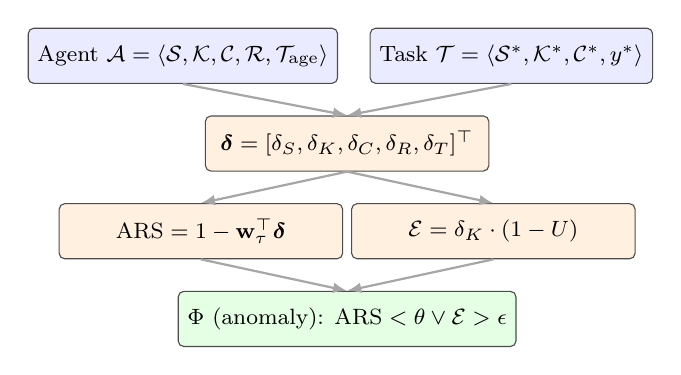
\begin{tikzpicture}[
  node distance=0.35cm and 0.4cm, font=\footnotesize,
  prof/.style={rectangle, draw=black!70, rounded corners=2pt,
               fill=blue!8, minimum width=2.6cm, minimum height=0.7cm, align=center},
  mm/.style={rectangle, draw=black!70, rounded corners=2pt,
             fill=orange!12, minimum width=3.6cm, minimum height=0.7cm, align=center},
  outbox/.style={rectangle, draw=black!70, rounded corners=2pt,
              fill=green!10, minimum width=3.6cm, minimum height=0.7cm, align=center},
  arr/.style={-{Latex[length=1.8mm]}, thick, gray!70},
]
  %% Top row: Agent and Task side by side
  \node[prof] (agent) {Agent $\A = \langle \Sk,\K,\CC,\R,\Tage\rangle$};
  \node[prof, right=of agent] (task) {Task $\T = \langle \Sk^*,\K^*,\CC^*,y^*\rangle$};
  %% Middle: mismatch vector centred under both
  \node[mm, below=0.4cm of $(agent.south)!0.5!(task.south)$] (delta)
       {$\boldsymbol{\delta}=[\delta_S,\delta_K,\delta_C,\delta_R,\delta_T]^\top$};
  %% Two parallel indicators
  \node[mm, below left=0.4cm and 0.05cm of delta.south] (ars)
       {$\ARS = 1 - \bw_\tau^\top\boldsymbol{\delta}$};
  \node[mm, below right=0.4cm and 0.05cm of delta.south] (eg)
       {$\E = \delta_K \cdot (1 - U)$};
  %% Final anomaly box centred at bottom
  \node[outbox, below=0.4cm of $(ars.south)!0.5!(eg.south)$] (phi)
       {$\Phi$ (anomaly): $\ARS<\theta \lor \E>\epsilon$};

  \draw[arr] (agent.south) -- (delta.north);
  \draw[arr] (task.south)  -- (delta.north);
  \draw[arr] (delta.south) -- (ars.north);
  \draw[arr] (delta.south) -- (eg.north);
  \draw[arr] (ars.south)   -- (phi.north);
  \draw[arr] (eg.south)    -- (phi.north);
\end{tikzpicture}
\caption{SKC reliability pipeline. Agent profile $\A$ and task profile
$\T$ produce a five-dimensional mismatch vector $\boldsymbol{\delta}$,
which feeds two parallel indicators: the Agent Reliability Score
($\ARS$) and the Epistemic Gap ($\E = \delta_K(1-U)$). The
anomaly-detection function $\Phi$ fires when either indicator crosses
its learned threshold.}
\label{fig:skc_pipeline}
\end{figure}

\section{Epistemic Gap}
\label{sec:epistemic}

The SKC model captures what an agent \textit{lacks}; the Epistemic Gap
captures what an agent \textit{thinks it has} versus what it actually has.
This distinction is critical for predicting hallucination, the most
dangerous failure mode in SOC environments.

\begin{definition}[Expressed Uncertainty]
  The expressed uncertainty $U(\A, \T) \in [0,1]$ is the complement of
  the confidence score the agent associates with its output:
  $U = 1 - \mathrm{conf}(\hat{y})$.
\end{definition}

\begin{definition}[Epistemic Gap]
  \begin{equation}
    \E(\A, \T) = \delta_K(\A, \T) \cdot (1 - U(\A, \T))
    \label{eq:epistemic_gap}
  \end{equation}
\end{definition}

Equation~\eqref{eq:epistemic_gap} formalises the \textit{confident ignorance}
failure mode. An agent with large knowledge deficit ($\delta_K \approx 1$)
that simultaneously reports high confidence ($U \approx 0$) produces
$\E \approx 1$: the maximal epistemic gap and the precondition for
hallucination. Conversely, an agent that correctly identifies its knowledge
limits ($U \approx 1$) produces $\E \approx 0$: it may fail the task but
will not fabricate an answer.

\begin{hypothesis}[Hallucination Precondition]
\label{hyp:hallucination}
  Hallucination probability $P_H$ is driven primarily by confident ignorance:
  $P_H \propto \E(\A, \T) = \delta_K \cdot (1 - U)$. This is empirically
  supported in Section~\ref{sec:experimental}.
\end{hypothesis}

\textbf{Connection to calibration theory.}
The Epistemic Gap operationalises findings from the confidence calibration
literature~\cite{guo2017calibration} for the specific case of agentic AI.
Modern neural networks are known to be systematically overconfident,
particularly on out-of-distribution inputs. The Epistemic Gap measures
whether this miscalibration occurs precisely where the agent's knowledge
is weakest: the most dangerous combination. A well-calibrated agent (one
whose confidence accurately reflects its accuracy) will produce low
$\E$ even under knowledge deficit, because it appropriately hedges its
outputs. This suggests that improving calibration in LLM-based security
agents may be as important as expanding their knowledge for reducing
dangerous failures.

\textbf{Why hallucination is particularly dangerous in SOC.}
An agent that says ``I don't have sufficient context'' is safe: it triggers
human escalation. An agent that confidently asserts a false threat
attribution is dangerous: it may trigger automated containment actions,
propagate fabricated IOCs to shared feeds, and erode analyst trust. The
Epistemic Gap captures exactly this distinction: it separates safe ignorance
(high $\delta_K$, high $U$, low $\E$) from dangerous confident ignorance
(high $\delta_K$, low $U$, high $\E$).

\textbf{Practical interpretation.}
Table~\ref{tab:eg_examples} illustrates the four quadrants of the Epistemic
Gap space with concrete SOC scenarios.

\begin{table}[t]
\caption{Epistemic Gap Quadrants with SOC Examples}
\label{tab:eg_examples}
\centering
\footnotesize
\setlength{\tabcolsep}{2.5pt}
\begin{tabular}{ccp{3.8cm}}
\toprule
$\delta_K$ & $U$ & \textbf{Scenario and Risk} \\
\midrule
Low  & Low  & Agent knows the threat and is confident. \textit{Safe: correct output likely.} \\
Low  & High & Agent knows but hedges. \textit{Suboptimal but safe: triggers review.} \\
High & High & Agent lacks knowledge and admits it. \textit{Safe: triggers escalation.} \\
High & Low  & Agent lacks knowledge but is confident. \textit{Dangerous: hallucination risk maximal ($\E \approx 1$).} \\
\bottomrule
\end{tabular}
\end{table}

The bottom-right quadrant (high $\delta_K$, low $U$, maximal $\E$) is
precisely where hallucination occurs: the agent does not possess the
knowledge required to answer correctly but proceeds with high confidence
regardless. The Epistemic Gap metric targets this quadrant specifically,
enabling monitoring systems to flag the most dangerous outputs before they
trigger automated actions.

\section{Experimental Illustration}
\label{sec:experimental}

\textbf{Testbed and dataset.} We evaluate \ARES{} on
\SAFK{}, a labelled corpus of $1{,}000$ agent execution traces produced by
the \ARESBench{} testbed under controlled mismatch injection. The corpus
contains $1{,}000$ executions in total: $750$ LLM-agent executions
(Mistral-7B-Instruct backbone) and $250$ rule-based control executions.
It spans four agent architectures (a single-agent LangGraph ReAct loop, a
three-stage AutoGen pipeline, a role-based CrewAI crew, and a rule-based
Sigma/YARA control) and five threat classes (Ransomware, Phishing, Insider
Threat, DDoS, APT Intrusion), with $250$ traces per architecture. Each trace records the task requirements
$\langle\Sk^*,\K^*,\CC^*\rangle$, the injected mismatch levels
$\delta_S,\delta_K,\delta_C \in \{0,\tfrac{1}{3},\tfrac{2}{3},1\}$, the
agent output, the agent's stated confidence, the failure label assigned by
the labelling pipeline, and the observed reliability outcome.
The corpus is split $600/200/200$ for training, validation, and held-out
test (stratified by task class and architecture).

\textbf{Labelling protocol.} Failure modes are first assigned by a
deterministic rule-based engine that compares each agent output against
the ATT\&CK-derived ground truth using a fixed codebook. We label five
manifestations: \textit{Hallucination} (output asserts facts that
contradict or are absent from the ground-truth incident),
\textit{Omission} (a required step is silently skipped),
\textit{Paralysis} (the agent halts because a required capability is
unavailable), \textit{Confabulation} (intermediate reasoning invents
nonexistent intermediate facts), and \textit{Overclaiming} (the agent
asserts coverage of TTPs or IOCs not present in the incident). A $10\%$
stratified sample ($n = 100$) is independently reviewed by two annotators;
inter-rater agreement is Cohen's $\kappa = 0.84$ for origin code and
$\kappa = 0.91$ for manifestation code, with disagreements resolved by
adjudication and rule-based labels revised to match human judgement in
$4.3\%$ of reviewed cases.

\subsection{Knowledge Mismatch Predicts Hallucination}

Across 750 LLM-based executions, hallucination rate increases monotonically
with $\delta_K$: from 1.4\% at $\delta_K = 0$ to 39.1\% at $\delta_K = 1.0$
(Fig.~\ref{fig:e1_isaia}). The Pearson correlation is $\rho = 0.92$
($p < 0.001$), strongly supporting Hypothesis~\ref{hyp:hallucination}. The
rule-based baseline exhibits zero hallucinations regardless of $\delta_K$,
confirming hallucination as an LLM-specific failure mode.

\begin{figure}[t]
\centering
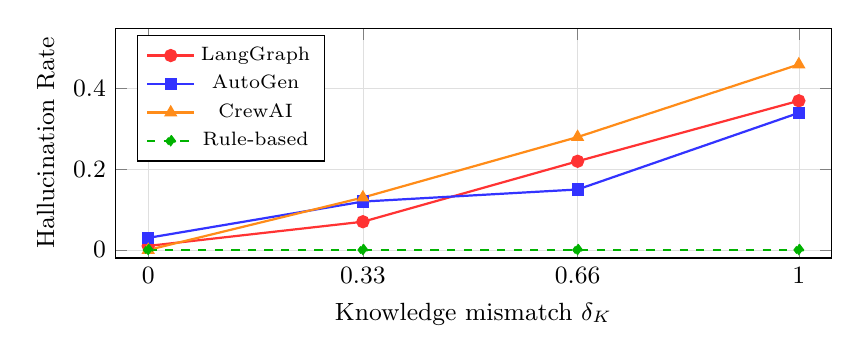
\begin{tikzpicture}
\begin{axis}[
  width=0.88\columnwidth, height=4.5cm,
  xlabel={Knowledge mismatch $\delta_K$},
  ylabel={Hallucination Rate},
  xmin=-0.05, xmax=1.05, ymin=-0.02, ymax=0.55,
  xtick={0,0.33,0.66,1.0},
  legend pos=north west,
  legend style={font=\scriptsize},
  grid=both, grid style={line width=0.2pt, draw=gray!25},
  tick label style={font=\small}, label style={font=\small},
]
\addplot[thick, color=red!80, mark=*, mark size=2]
  coordinates {(0,0.01)(0.33,0.07)(0.66,0.22)(1.0,0.37)};
\addlegendentry{LangGraph}
\addplot[thick, color=blue!80, mark=square*, mark size=1.8]
  coordinates {(0,0.03)(0.33,0.12)(0.66,0.15)(1.0,0.34)};
\addlegendentry{AutoGen}
\addplot[thick, color=orange!90, mark=triangle*, mark size=2]
  coordinates {(0,0.00)(0.33,0.13)(0.66,0.28)(1.0,0.46)};
\addlegendentry{CrewAI}
\addplot[thick, color=green!70!black, mark=diamond*, mark size=2, dashed]
  coordinates {(0,0.0)(0.33,0.0)(0.66,0.0)(1.0,0.0)};
\addlegendentry{Rule-based}
\end{axis}
\end{tikzpicture}
\caption{Hallucination Rate vs.\ knowledge mismatch $\delta_K$ across
four agent architectures ($n = 750$ LLM executions).}
\label{fig:e1_isaia}
\end{figure}

\subsection{Framework-Level Results}

We summarise four additional framework-level results.

\textbf{ARS threshold generalisation.} The optimal ARS threshold
($\theta^* = 0.58$), learned via isotonic regression on the training
split, achieves test F1 $= 0.96$ (precision $1.00$, recall $0.92$)
with the minimum per-class test F1 at $0.91$ and a one-point
train--test gap. A stricter leave-one-threat-class-out protocol
recovers mean test F1 $= 0.957$, supporting ARS as a generalisable
reliability signal rather than a class-memorising score.
The reported threshold result uses the post-execution ARS including
$\delta_R$; $\ARS^{\mathrm{pre}}$ is intended for pre-execution
screening and showed the same directional trend but lower absolute
discrimination because reasoning mismatch is unavailable before
execution.

\textbf{Distinct failure signatures per mismatch dimension.} Isolating
each mismatch dimension at $\delta = 0.66$ yields diagnostically
separable manifestation distributions (chi-square $= 146.7$,
$p < 0.001$, dof $= 18$): capability deprivation predominantly
produces Paralysis ($76\%$), skill deficit produces silent
Omission ($60\%$), and reasoning perturbation produces
Confabulation plus Overclaiming ($77\%$ combined) -- the most
dangerous signature because confidence-inflated errors are the most
likely to mislead downstream consumers.

\textbf{Cascade degradation.} The naive head-line gap between AUT-1
(single-agent LangGraph) and AUT-2 (three-stage AutoGen pipeline) is
$\sim 5.7\%$ relative ARS (mean ARS $0.659$ vs.\ $0.621$), but this
conflates framework identity with pipeline depth. A controlled
ablation on $27$ strictly matched mismatch buckets isolates the two
contributions: framework identity contributes $\mathbf{0.13\%}$
(essentially zero) and pure pipeline depth contributes
$\mathbf{17.25\%}$. The pipeline-depth effect is consistent across
all five threat classes and empirically supports
Theorem~\ref{thm:cascade} in the tightly-coupled regime, where the
empirical $\mu^*_{\max} \geq 0.8$ in $100\%$ of AUT-2 records.

\textbf{Epistemic Gap as interpretable decomposition.} Epistemic Gap
and raw knowledge mismatch achieve statistically indistinguishable
correlation with false-negative severity
($\rho_\mathcal{E} = 0.80$ vs.\ $\rho_{\delta_K} = 0.80$, Fisher
$z$-test $p = 0.78$). The value of $\mathcal{E}$ is decomposing risk
into a knowledge term ($\delta_K$) and a calibration term ($1 - U$),
exposing two independently mitigable axes. A 30-incident validation
against the live CISA KEV catalogue (post-training-cutoff, so
$\delta_K \approx 1$) yields an operational $\E$ gap of $\sim 66\%$
at matched $\delta_K$ across five frontier LLM backbones.

\textbf{Cross-model-family generalisation.} The
hallucination-versus-$\delta_K$ relationship replicates directionally
across four LLM families from 7B (Mistral-7B-Instruct) to frontier
scale (GPT-4o-mini, Claude Haiku~4.5, Claude Sonnet~4.6), with
bucket-aggregated $\rho \in [0.78, 0.95]$; absolute thresholds require
per-model recalibration.

Together with the knowledge-hallucination relationship in
Fig.~\ref{fig:e1_isaia}, these results indicate that \ARES{} captures
meaningful, generalisable reliability signals across diverse agent
architectures and threat scenarios.

\section{Discussion}
\label{sec:discussion}

\subsection{Implications for AI System Evaluation}

The \ARES{} framework provides a principled basis for evaluating AI agent
reliability \textit{before deployment}. Because four of the five mismatch
dimensions ($\delta_S$, $\delta_K$, $\delta_C$, $\delta_T$) are computable
from the agent's declared profile and the task's requirements alone, ARS
can serve as a pre-execution deployment gate: agents scoring below $\theta^*$
are automatically escalated to human analysts rather than executing
autonomously. This approach is consistent with the NIST AI Risk Management
Framework~\cite{nist_ai_rmf}, which recommends continuous monitoring of AI
system performance against operational requirements.

The task-class-specific weight vectors (Table~\ref{tab:weights_isaia})
provide additional operational value: they reveal which capability
dimensions matter most for each threat type. A SOC deploying an agent for
ransomware detection should prioritise knowledge coverage ($w_K = 0.35$),
while an agent assigned to DDoS mitigation should be evaluated primarily
on skill and capability access ($w_S + w_C = 0.60$). This dimension-specific
guidance enables targeted agent improvement rather than generic capability
enhancement.

\subsection{Trustworthy Deployment of AI Agents}

The Epistemic Gap metric supports runtime monitoring of hallucination
risk: by comparing an agent's stated confidence against its known
knowledge coverage, organisations can flag high-risk outputs for human
review before they trigger automated actions. The temporal drift model
($\delta_T$) provides a quantitative basis for scheduling knowledge
updates -- e.g., for high-volatility domains like ransomware
($\lambda = 0.005$), ARS degrades below $\theta^*$ in approximately
$120$ days, suggesting a quarterly refresh cycle. The cascade
reliability bound (Theorem~\ref{thm:cascade}) implies that decomposing
a task into a tightly-coupled pipeline cannot improve reliability beyond
the weakest agent, so single-agent designs should be preferred for
critical tasks unless per-agent reliability is independently verified.

\subsection{Limitations}

\textbf{LLM specificity.} Experiments use Mistral-7B-Instruct; absolute
thresholds will require recalibration for larger models, though directional
findings should hold since the SKC model is architecture-agnostic.
\textbf{Linear formulation.} The additive ARS is chosen for
interpretability and decomposability; nonlinear alternatives may improve
predictive power at the cost of transparency.
\textbf{Synthetic data.} The dataset is generated from ATT\&CK and NVD;
real-world SOC incidents introduce additional noise and ambiguity.
\textbf{Cascade model.} The formulation assumes acyclic pipelines and
independent mismatch factors; cyclic architectures and correlated
dimensions require further modelling.
\textbf{Controlled benchmark.} Because the benchmark uses controlled
mismatch injection, real SOC deployments may exhibit noisier and
less separable failure patterns.

\section{Conclusion}
\label{sec:conclusion}

We presented \ARES{}, a compact formal reliability framework for
detecting anomalous behaviour in agentic AI systems deployed in
cybersecurity environments. The conference contribution is narrow:
the SKC mismatch model produces a learnable ARS that generalises
across threat classes (test F1 0.96), and the Epistemic Gap
metric formalises the hallucination precondition as
\textit{confident ignorance} and decomposes false-negative risk into
knowledge and calibration components. A cascade reliability bound for
tightly-coupled pipelines and a temporal-drift model for knowledge
ageing are reported as supporting results.

Practically, ARS supports pre-deployment reliability screening, the
Epistemic Gap supports runtime hallucination-risk monitoring, the
temporal-drift model supports evidence-based knowledge maintenance, and
the cascade bound informs conservative multi-agent design, an initial
formal foundation for trustworthy agentic AI in cybersecurity that may
generalise to other domains where autonomous agents decide under
incomplete knowledge.

Future work follows the limitations above. The most consequential step
is to move from controlled injection to measurement: recovering the
mismatch dimensions from live agents in a production SOC, where
$\delta_K$ and expressed uncertainty must be read from real telemetry
rather than set by construction. Companion work takes a first step for
the knowledge and calibration terms, and early results there suggest
that agent calibration, not knowledge coverage alone, governs whether a
mismatch becomes a dangerous failure. Cyclic multi-agent architectures
and adversarial mismatch injection remain open. The \SAFK{} corpus and
evaluation testbed are released
publicly.\footnote{Project page: \url{https://github.com/IntelEyes/ARES-Framework}}


\bibliographystyle{IEEEtran}
\bibliography{references}

\end{document}
